%!TEX root = report.tex

\chapter{Appendix} % (fold)
\label{cha:appendix}

\section{NX Advanced Simulation Guide} % (fold)
\label{sec:nx_advanced_simulation_guide}
TODO: Put guide here.

% \begin{figure}[t]
% 	\begin{center}
% 		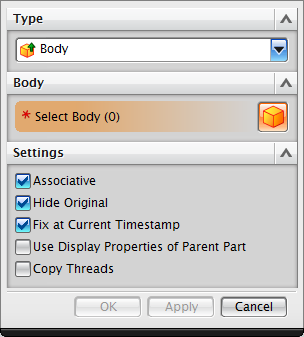
\includegraphics{WAVEGeometryLinker}
% 	\end{center}
% 	\caption{WAVE Geometry Linker dialogue box in NX.}
% 	\label{fig:WAVEGeometryLinker}
% \end{figure}
% section nx_advanced_simulation_guide (end)

\section{\texttt{CreateGroups}} % (fold)
\label{sec:creategroups}
\lstinputlisting[language=Python]{codesnippets/creategroups.py}
\subsection{\texttt{GetNXGroups}} % (fold)
\label{sub:getnxgroups}
\lstinputlisting[language=Python]{codesnippets/getnxgroups.py}
% subsection getnxgroups (end)
% section creategroups (end)

\section{\texttt{CreateMesh}} % (fold)
\label{sec:createmesh}
\lstinputlisting[language=Python]{codesnippets/createmesh.py}
\subsection{\texttt{CreateAlgorithm}} % (fold)
\label{sub:createalgorithm}
\lstinputlisting[language=Python]{codesnippets/createalgorithm.py}
% subsection createalgorithm (end)
% section createmesh (end)

\section{\texttt{PartitionShapes}} % (fold)
\label{sec:partitionshapes}
\lstinputlisting[language=Python]{codesnippets/partitionshapes.py}
\subsection{CreateTreeStructure} % (fold)
\label{sub:createtreestructure}
\lstinputlisting[language=Python]{codesnippets/createtreestructure.py}
% subsection createtreestructure (end)
\subsection{MoveContactGroups} % (fold)
\label{sub:movecontactgroups}
\lstinputlisting[language=Python]{codesnippets/movecontactgroups.py}
% subsection movecontactgroups (end)
\subsection{MoveOtherGroups} % (fold)
\label{sub:moveothergroups}
\lstinputlisting[language=Python]{codesnippets/moveothergroups.py}
% subsection moveothergroups (end)
% section partitionshapes (end)

\section{\texttt{CreateSubMesh}} % (fold)
\label{sec:createsubmesh}
\lstinputlisting[language=Python]{codesnippets/createsubmesh.py}
% section createsubmesh (end)

% chapter appendix (end)